\section{Mercado de Trabalho}
%%%%%%%%%%%%%%%%%%%%%%%%%%%%%%%%%%%%%%%%%%%%%%%%%%%%%%%%%%%%%%%%
\begin{frame}
\frametitle{\textcolor{green}{O que é dinheiro ?}}
\textsc{\large Dinheiro é uma representação de valore, é o teu trabalho, os teus valores e competências, tudo que representas a não ser que sejas político.}\\
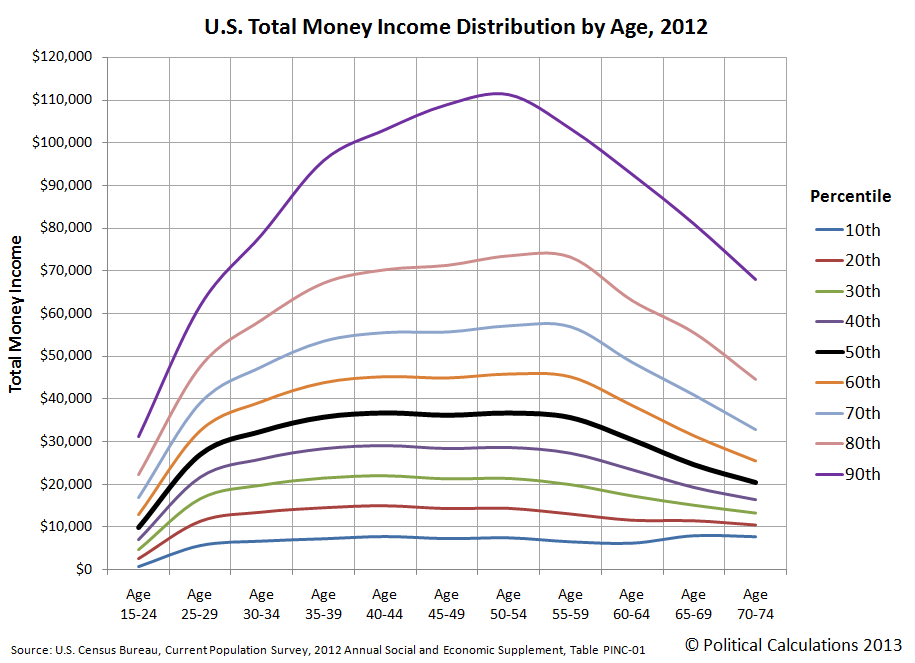
\includegraphics[scale=0.2]{./image/Career_Path/Income_2012}\hspace{0.8cm}
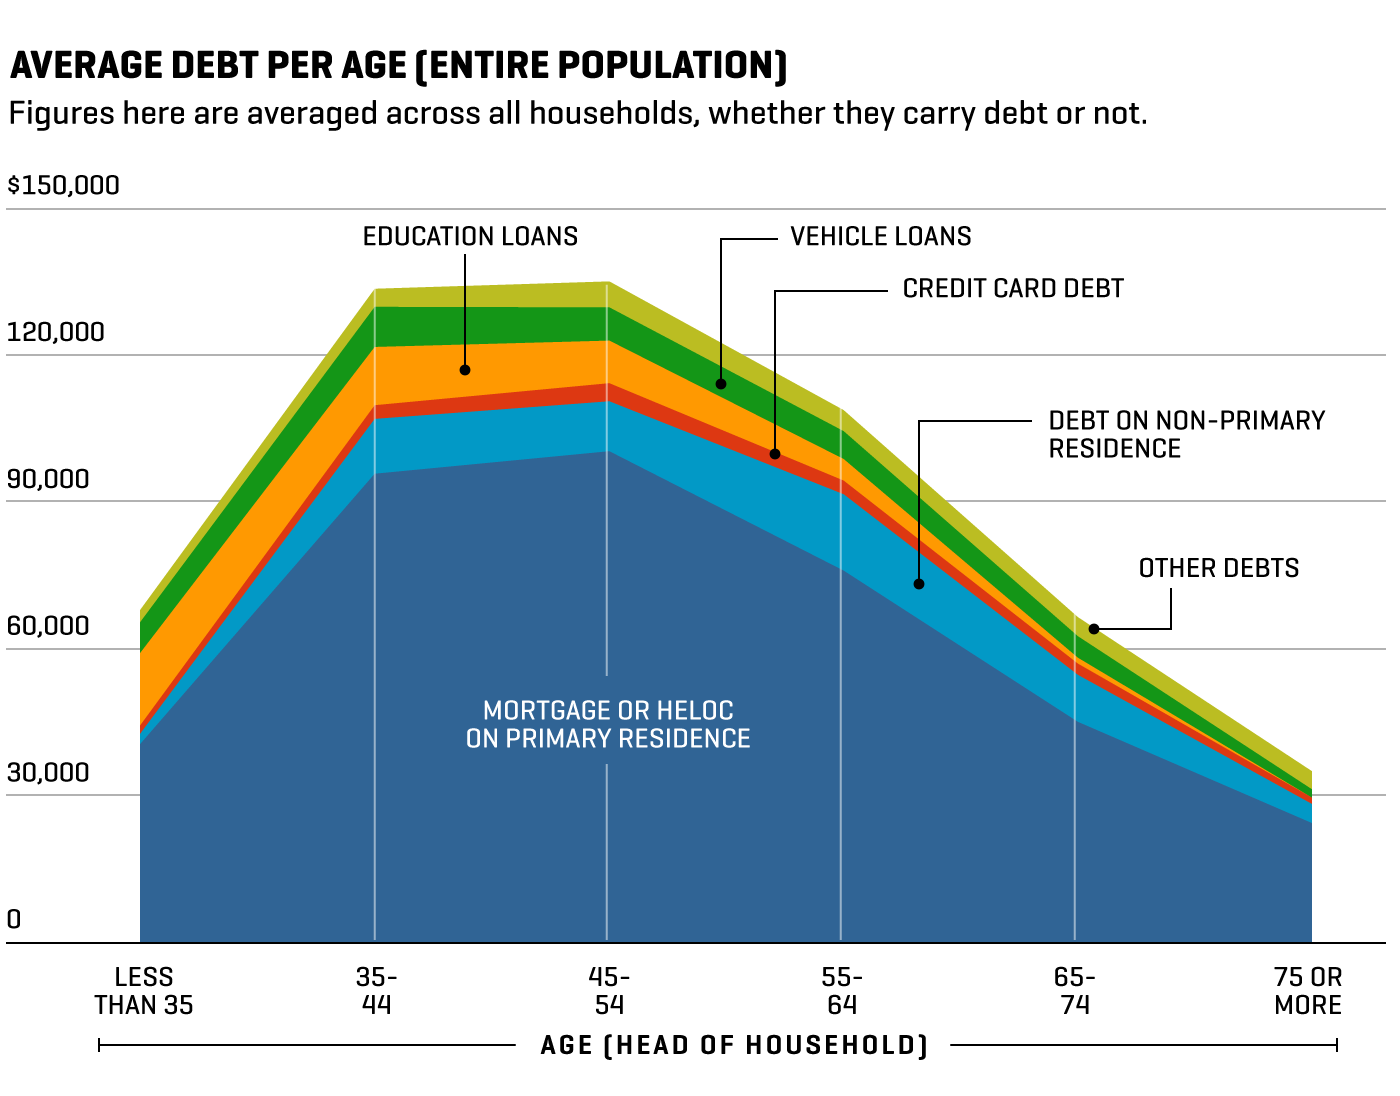
\includegraphics[scale=0.125]{./image/Career_Path/Debt}
\end{frame}
%%%%%%%%%%%%%%%%%%%%%%%%%%%%%%%%%%%%%%%%%%%%%%%%%%%%%%%%%%%%%%%%
\begin{frame}
\frametitle{\textcolor{green}{Porque Dinheiro ?}}
\begin{itemize}
	\item \textbf{Portabilidade} \\
	Reconhecido internacionalmente, sendo que cada pais tem uma cotação de valore de mercado, sendo o Pound, Dólar ,Euro e Yuan as mais fortes, em ordem decrescente, e o dólar a moeda de cambio internacional até agora.
	\item \textbf{Avaliação} \\
	Por isso que na escola os teus resultados são notas.\\
	Portugal pertence a Europa, mas um Português tem menos valor que um Alemão, Francês, Italiano e Espanhol, a não ser que sejas Político Português.\\Um Euro vale 7,69 Yuan, pelo menos um chinês vale sete vezes menos que um Europeu.\\
	\item \textbf{Modernização} \\
	Das cavernas a sobreviver do ambiente, a troca de bens, e ao cambio por moeda.
\end{itemize}
\end{frame}
%%%%%%%%%%%%%%%%%%%%%%%%%%%%%%%%%%%%%%%%%%%%%%%%%%%%%%%%%%%%%%%%
\begin{frame}
\frametitle{Valorização Pessoal}
\begin{center}
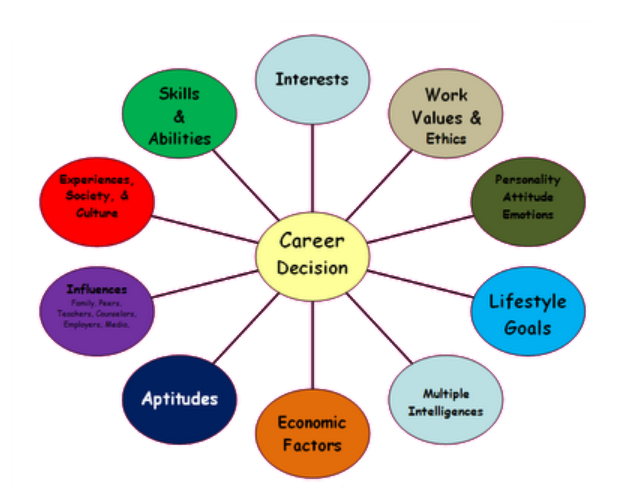
\includegraphics[scale=0.4]{./image/Career_Path/Career_Decision_Factors}
\end{center}
\end{frame}
%%%%%%%%%%%%%%%%%%%%%%%%%%%%%%%%%%%%%%%%%%%%%%%%%%%%%%%%%%%%%%%%
